\section{Packrat Protocol}
\label{sec:packrat-protocol}

The \Sys protocol is spoken between a client and an on-path proxy, where the
client is a data \textit{receiver}. We imagine the proxy to exist near the data
receiver on the other side of a lossy path segment. This could be as close as
directly behind a Wi-Fi access point, at a cellular base station, or on the
first extraterrestrial node of a satellite network path. This is on the order
of 1s to 10s of milliseconds.

As an overview, once the client and proxy have established an adjacent
connection for a specific base connection identified by a UDP 4-tuple, the
proxy is ready to send in-network retransmissions. The client sends
acknowledgements of which encrypted packets it has received, and the proxy retransmits missing
packets it previously forwarded on that base connection.
But in-network retransmissions are not just that simple.

In the rest of this section, we start by describing the \textit
{reordering problem} with in-network retransmissions, and a mechanism at
the \textit{client} to address the issue. Then we describe the messages
exchanged between the client and proxy in the \Sys protocol to establish the
adjacent connection and generate in-network retransmissions,
and the behavior of each party in both the \Sys and base
connections. We assume each message is transmitted in an unreliable UDP
datagram.

\subsection{The Reordering Problem}
\label{sec:packet-protocol:problem}

\begin{figure}
    \centering
    \begin{subfigure}[b]{0.8\linewidth}
        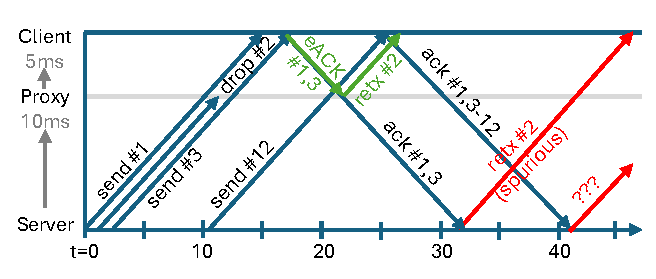
\includegraphics[width=\linewidth, trim=0 10 0 10, clip]{figures/reordering_unmodified.pdf}
        \caption{Unmodified ACK.}
        \label{fig:reordering-problem:unmodified}
    \end{subfigure}
    \begin{subfigure}[b]{0.8\linewidth}
        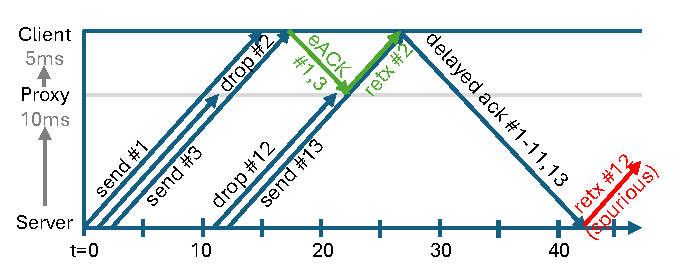
\includegraphics[width=\linewidth, trim=0 9 0 10, clip]{figures/reordering_delayed_ack.pdf}
        \caption{Na\"ive delayed ACK.}
        \label{fig:reordering-problem:delayed-ack}
    \end{subfigure}
    \begin{subfigure}[b]{0.8\linewidth}
        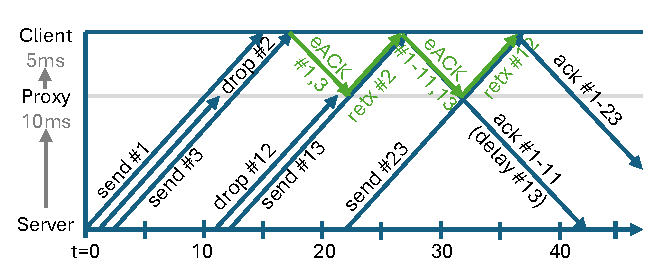
\includegraphics[width=\linewidth, trim=0 9 0 10, clip]{figures/reordering_with_signal.pdf}
        \caption{ACK with \Sys reorder delay of 10 ms.}
        \label{fig:reordering-problem:packrat}
    \end{subfigure}
    \caption{\small The reordering problem where in-network retransmissions with
    millisecond RTTs cause the server to send spurious retransmissions. The
    end-to-end ACKs constructed with a \Sys reorder delay prevent this problem.
    \vspace{-0.4cm}
    }
    \label{fig:reordering-problem}
\end{figure}

Most acknowledgment schemes allow for some reordering but not at the level
incurred by in-network retransmissions. For example, TCP fast retransmit requires
three duplicate ACKs~\cite{rfc5681tcp}. The QUIC RFC specifies a threshold of three
out-of-order packets before detecting loss~\cite{rfc9002quic}. The RACK-TLP algorithm
allows for a time-based ``reordering window'', but still penalizes excessive
reordering~\cite{rfc8985}. Compared to, e.g., Wi-Fi retransmits, the
reordering from in-network transmissions is directly related to the RTT to
the proxy on the order of tens of milliseconds.
We call this the \textit{reordering problem}.

Consider an example using selective ACKs, where a gap is considered a missing
packet (\Cref{fig:reordering-problem:unmodified}): The server sends 1250-byte packets at 10 Mbit/s,
which is 1 packet every ms. The client drops packet \#2 but
receives \#1, \#3, \#4, etc. If the RTT between the client and proxy is 10 ms,
by the time the client receives the in-network retransmission of \#2 (from
eACKing \#1 and \#3), it could
have already ACKed $10$ more packets with higher sequence
numbers up to \#12. The server unnecessarily retransmits \#2 and treats the
loss as a congestion signal.
Spurious retransmissions take up valuable bandwidth and confuse congestion
control algorithms~\cite{leung2007overview}.

\paragraph{Na\"ive solutions.}

The Snoop protocol faces the same challenges with needing to modify end-to-end
signals when sending in-network retransmissions~\cite
{balakrishnan1995snoop}. The solution here involves withholding duplicate TCP
ACKs from the server if the proxy has the packet in the cache. However, without
plaintext sequence numbers, the \Sys proxy is unable to understand which
encrypted packets an encrypted end-to-end ACK is referring to, and can only
forward packets as intended.

Another option may be for the client to \textit{delay} sending an ACK until it
has allowed one proxy RTT for the proxy to retransmit the packet first~\cite{rfc3168}.
In the
previous example, the client may wait 10 ms from detecting the gap in
packet \#2 before sending an ACK, at which point it would have received the
retransmission for \#2 and be able to ACK the full range from \#1-13. This
seems promising at first, but in the time the client was waiting,
another loss could have occurred (\#12)
and the new ACK would have the same problem (\Cref{fig:reordering-problem:delayed-ack}).

Various other solutions exist, such as changing a server configuration, but it
is also undesirable to require certain features in all data senders as they
should not have to participate in the \Sys protocol.
% Various other na\"ive solutions exist, such as informing the server to increase
% its reordering threshold, but this requires it to be a configurable parameter
% in the base protocol. It is also undesirable to require certain features in all
%  data senders, as they should not have to participate in the \Sys protocol.

\paragraph{\Sys solution.}

Our solution is for the end-to-end ACKs constructed by the client to
signal \textit{jitter}, defined as variation in packet interarrival times,
instead of reordering. This enables the data receiver to process packets as
soon as they are received and reduces spurious retransmissions from the data
sender, without involving the data sender. The precise manifestation depends on
the acknowledgment scheme.

For example, QUIC ACKs consist of a cumulative sequence number, followed by SACK
ranges. Using \Sys, the QUIC ACK instead includes the cumulative sequence
number, but then only the ranges for packets that have been received for at
least the time it takes for the proxy to retransmit. This
\textit{reorder delay} includes the RTT to the proxy
as well as any delay in sending the eACK.
In the example, 10 ms after detecting the gap in \#2, the ACK consists
of packets \#1-2 and any cumulative sequence numbers beyond \#2 (up to \#11)
(\Cref{fig:reordering-problem:packrat}).
We assume
that most loss is near the client, and that the RTT to the proxy is less than
the loss detection timeout.

Different protocols use different acknowledgment schemes with similar flavors.
The modification for negative acknowledgments of missing packets is to delay
sending the NACK for at least one proxy RTT before deciding whether the NACK is
still needed. TCP relies on duplicate ACKs, which need a different
modification. Abstractly, packets are held and ordered in a jitter buffer for a
certain delay before they can be referenced in the client's underlying
acknowledgments.

% To do so, we give the proxy a chance to react to missing packets on that path
% segment by delaying the positive ACK signal until it has had two cycles to
% retransmit. The algorithm is as follows: If there is a consecutive sequence
% number, retransmit. If not, ACK packets in the SACK range only if they have
% been received for at least this threshold. This ensures that if the ACK will
% not trigger a retransmission, we send it. In the case of QUIC, we adjust the
% ACK delay and largest acknowledged accordingly.

% What are the consequences from the data sender perspective? It will think that
% some packets are delayed when there is truly a loss, though below the loss
% detection threshold. If there are losses it is truly responsible for, it will
% fall back to this end-to-end retransmission mechanism. If most losses are in
% this path segment near the data receiver, it may think that the RTT is
% unusually long.

% \paragraph{Modified NACKs.} In the case of negative acknowledgments, stating
%  which packets have likely been lost, we can just withhold that signal for a
%  certain delay.


\subsection{Handshake}

\newtcolorbox{protopayload}[2][]{
  colback=yellow!20,
  colframe=black,
  boxrule=0.5pt,
  arc=1pt,
  fontupper=\ttfamily,
  width=\linewidth,
  fonttitle=\small\bfseries,
  top=-1.5mm,
  bottom=-1.5mm,
  left=2mm,
  right=2mm,
  title={#2},
  #1
}

\begin{figure}[t]
    % \centering
    % Client payloads
    \begin{subfigure}[b]{0.48\linewidth}
        \begin{protopayload}{\texttt{Init}}
            \begin{lstlisting}[language=Rust,basicstyle=\footnotesize]
epoch: u32;
base_conn: [u8; 12];
eack_ty: u8;
num_symbols: u8;
id_offset: u16;
mem_bytes: u32;
            \end{lstlisting}
        \end{protopayload}
        \begin{protopayload}{\texttt{quACK}}
            \begin{lstlisting}[language=Rust,basicstyle=\footnotesize]
count: u32;
last_identifier: u32;
code: Vec<Symbol>;
            \end{lstlisting}
        \end{protopayload}
        \caption{Client payloads.}
        \label{fig:payloads:client}
    \end{subfigure}
    \hfill
    % Proxy payloads
    \begin{subfigure}[b]{0.48\linewidth}
        \begin{protopayload}{\texttt{InitACK}}
            \begin{lstlisting}[language=Rust,basicstyle=\footnotesize]
epoch: u32;
udp_port: u16;
errno: u32;
            \end{lstlisting}
        \end{protopayload}
        \begin{protopayload}{\texttt{Reset}}
            \begin{lstlisting}[language=Rust,basicstyle=\footnotesize]
epoch: u32;
errno: u32;
            \end{lstlisting}
        \end{protopayload}
        \begin{protopayload}{\texttt{Retransmit}}
            \begin{lstlisting}[language=Rust,basicstyle=\footnotesize]
udp_payload: Vec<u8>;
            \end{lstlisting}
        \end{protopayload}
        \caption{Proxy payloads.}
        \label{fig:payloads:proxy}
    \end{subfigure}
  % Caption
  \caption{Packrat protocol messages to initialize the connection and generate
   retransmissions. There are two constructions of the quACK: power sum and
   IBLT (\Cref{sec:quack}). The \texttt{Symbol} uses 5 and 4 bytes in each
   type, respectively.}
  \label{fig:payloads}
\end{figure}


Now we describe the messages that are exchanged in the
\Sys protocol (\Cref{fig:payloads}), starting with the handshake.

\Sys\!s are distinguished from other types of proxies such as VPNs and
transparent PEPs in that the proxy is on the path and the client is knowingly
receiving in-network retransmissions. In order to discover \Sys proxies on the
path, the client sends a magic discovery packet along the base connection
4-tuple, after it has established that connection. Proxies respond by
announcing that they support \Sys and their supported configurations, and the
server discards the invalid magic packet. Clients can choose to accept
assistance from a proxy by replying with an \texttt{Init} and their
configuration request. The proxy completes the handshake with an \texttt
{InitACK} and a new UDP address specific to this base connection.

The client configuration in \texttt{Init} includes several parameters (\Cref
{fig:payloads:client}). This includes: the type of encoding used for the eACK,
the number of symbols to use in the encoding, the byte offset in the randomly
encrypted payload at which to parse the 4-byte identifier, and the size of the
requested cache. The client may dynamically adjust these configurations with
new \texttt{Init} packets as it learns more about the network path.

The proxy accepts or rejects these configurations with an \texttt{InitACK}, and
is ready to cache packets and retransmit. On receiving an \texttt{InitACK}, the
client is free to send eACKs.

\subsection{Client Behavior}

In addition to modifying end-to-end acknowledgments to avoid sending excessive
reordering signals to the server, the primary behavior of the client is
to \texttt{eACK} at a specified frequency, e.g., every 10 ms or every 16
packets. This frequency is typically the same as that of the underlying
acknowledgment scheme. The eACKs are cumulative representations of all the
packets ever received since sending the last \texttt{Init}.

% In the remainder of this section, we describe how we modify the client's
% behavior in the base connection to avoid sending excessive reordering signals
% to the server.

\subsection{Proxy Behavior}
\label{sec:packrat-protocol:proxy-behavior}

The behavior of the proxy is to decode incoming eACKs and retransmit missing
packets, and to cache and evict packets from the base connection for
retransmission. The state at the proxy for each base connection is (1) a packet
cache and (2) an eACK that represents the cumulative encoding of all packets
received by the client that are no longer in the cache.

\paragraph{Decode eACKs and retransmit.}

The \texttt{eACK} definitively states which packets have been \textit{received}
by the client. Based on its knowledge of which packets it has \textit{sent} to
the client, the proxy evicts any newly received packets from the cache. The
proxy then applies a loss detection policy to determine which of its sent
packets may have been dropped. The default
policy is any ``gap" in the ordered sequence of packets that were previously
cached, but packet timeouts could also apply. The proxy immediately retransmits
these missing packets, moving them to the top of the cache.

The retransmission is simply a duplicate of the original packet on the wire.
However, the proxy can also explicitly indicate that the retransmission comes
from the \Sys by encapsulating the UDP payload in a \texttt{Retransmit}. The
packet would be received by the client on the \Sys socket, which can then forward
the payload to the base connection.

\paragraph{Cache and evict packets.}

The proxy caches packets with the base connection 4-tuple in the order they are
forwarded to the client, up to the pre-configured cache size. It evicts packets
if an \texttt{eACK} indicates they have been received and no longer need to be
retransmitted. Whenever a packet is evicted, it is also encoded in the eACK
state of the base connection.

If a packet of the base connection arrives but the cache is full, the
proxy \textit{optimistically} evicts the oldest packets to make room. When
retransmissions are uncommon, this allows the client to eACK less frequently
and the proxy to maintain a significantly smaller cache. Unlike
connection-splitters, the proxy does not actually make reliability \textit
{guarantees}, and the client can always fall back to end-to-end retransmissions
after resetting the \sys connection, as described below.

\paragraph{Reset the \sys connection.}

If the proxy is unable to decode a eACK for any reason, it sends a \texttt
{Reset} to the client. These reasons include but are not limited to: an
insufficient number of symbols to decode the missing packets, a necessary
retransmission was optimistically evicted,
a packet corruption caused the encoded identifiers
to become out of sync, etc. The \texttt{Reset} indicates the start of a new
epoch in which the client and proxy encode identifiers into their eACKs.

Base connections that use the \Sys protocol must always be able to fall back to
end-to-end mechanisms when the \Sys is unable to send in-network
retransmissions. This is unlike typical connection-splitters and VPNs that fate
share with their endpoints. Similar to Snoop~\cite{balakrishnan1995snoop},
the \Sys style of in-network
assistance is better suited to mobility and handoffs if the connection ever
changes network paths.

% \subsection{Multicast Proxy}

% \Sys connections share the same base connection for a multicast address, and the
% Discovery packet additionally indicates that it is a multicast address. In
% this case, it is necessary to use the Retransmit payload to sends messages, to
% avoid multicasting the entire retransmission.

% We want to keep the same underlying packet buffer for each \sys connection,
% since they share the same packet stream. What makes it challenging is that if
% we retransmit packets for a certain \sys connection, they are technically
% reordered in the packet buffer.

% We overcome this by keeping a \textit{virtual} packet buffer for each \sys
% connection pointing to indexes in the original packet buffer. There is
% additional state proportional to the number of in-flight retransmitted packets,
% indicating where these packets are ``reinserted'' into the virtual buffer.
% However, we can still traverse the packet buffer $O(1)$ for each packet as
% necessary.

% Eviction for the underlying cache ensures the original packet payload stays
% around while it is still in-flight. If the proxy reaches a memory limit, it can
% send a Reset packet to those connections that are preventing eviction.
